\let\negmedspace\undefined
\let\negthickspace\undefined
\documentclass[journal,12pt,onecolumn]{IEEEtran}
\usepackage{cite}
\usepackage{amsmath,amssymb,amsfonts,amsthm}
\usepackage{algorithmic}
\usepackage{graphicx}
\graphicspath{{./figs/}}
\usepackage{textcomp}
\usepackage{xcolor}
\usepackage{txfonts}
\usepackage{listings}
\usepackage{enumitem}
\usepackage{mathtools}
\usepackage{gensymb}
\usepackage{comment}
\usepackage{caption}
\usepackage[breaklinks=true]{hyperref}
\usepackage{tkz-euclide} 
\usepackage{listings}
\usepackage{gvv}                                        
%\def\inputGnumericTable{}                                 
\usepackage[latin1]{inputenc}     
\usepackage{xparse}
\usepackage{color}                                            
\usepackage{array}                                            
\usepackage{longtable}                                       
\usepackage{calc}                                             
\usepackage{multirow}
\usepackage{multicol}
\usepackage{hhline}                                           
\usepackage{ifthen}                                           
\usepackage{lscape}
\usepackage{tabularx}
\usepackage{array}
\usepackage{float}
%\newtheorem{theorem}{Theorem}[section]
%\newtheorem{theorem}{Theorem}[section]
%\newtheorem{problem}{Problem}
%\newtheorem{proposition}{Proposition}[section]
%\newtheorem{lemma}{Lemma}[section]
%\newtheorem{corollary}[theorem]{Corollary}
%\newtheorem{example}{Example}[section]
%\newtheorem{definition}[problem]{Definition}

\begin{document}

\title{1.9.9}
\author{EE25BTECH11020 - Darsh Pankaj Gajare}
% \maketitle
% \newpage
% \bigskip
%\begin{document}
{\let\newpage\relax\maketitle}
%\renewcommand{\thefigure}{\theenumi}
%\renewcommand{\thetable}{\theenumi}
Question:\\
Find the distance between the points $\vec{A}\brak{-\frac{7}{3},5}$ and $\vec{B}\brak{\frac{2}{3},5}$.\\
\textbf{Solution:}
\begin{table}[H]
	\centering
	\begin{center}
    \begin{tabular}{|c|c|c|} 
        \hline
            \textbf{Variable} & \textbf{Parameter} & \textbf{Value} \\ 
        \hline
            $\lVert \vec{B - A}\rVert$ & c & 5 cm \\ 
        \hline
             $\lVert \vec{C - B}\rVert$ & a & - \\ 
        \hline
             $\lVert \vec{C - A}\rVert$ & b &   -    \\
        \hline
            $\angle \vec{A}$  & -  & $45^\circ$ \\
        \hline
    \end{tabular}
\end{center}  

	\caption{Given Data}
	\label{}
\end{table}
\begin{align}
	\because \vec{A}-\vec{B}=\myvec{-\frac{7}{3}\\5}-\myvec{\frac{2}{3}\\5}=\myvec{-3\\0},
\end{align}
\begin{align}
	\brak{\vec{A}-\vec{B}}^T\brak{\vec{A}-\vec{B}}=9
\end{align}
Thus, the desired distance is
\begin{align}
	d=\norm{\vec{A}-\vec{B}}=3
\end{align}
\begin{figure}[H]
	\centering
	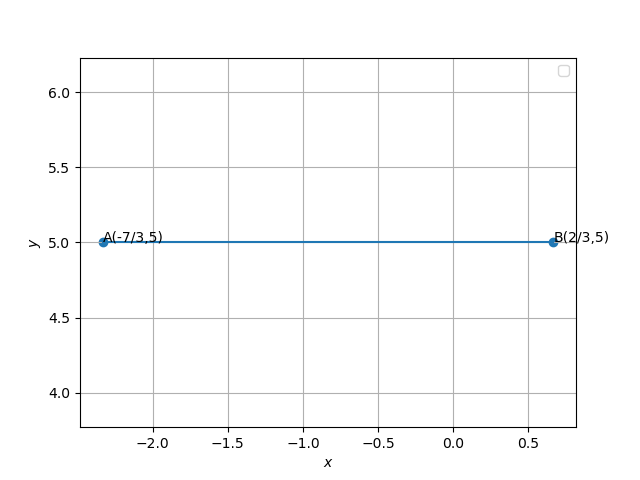
\includegraphics[scale=0.5]{img}
	\caption*{}
	\label{img}
\end{figure}
\end{document}
